%% 
%% Copyright 2007, 2008, 2009 Elsevier Ltd
%% 
%% This file is part of the 'Elsarticle Bundle'.
%% ---------------------------------------------
%% 
%% It may be distributed under the conditions of the LaTeX Project Public
%% License, either version 1.2 of this license or (at your option) any
%% later version.  The latest version of this license is in
%%    http://www.latex-project.org/lppl.txt
%% and version 1.2 or later is part of all distributions of LaTeX
%% version 1999/12/01 or later.
%% 
%% The list of all files belonging to the 'Elsarticle Bundle' is
%% given in the file `manifest.txt'.
%% 
%% Template article for Elsevier's document class `elsarticle'
%% with harvard style bibliographic references
%% SP 2008/03/01

%\documentclass[preprint,12pt,authoryear]{elsarticle}  %default in the template
%\documentclass[preprint,10pt,authoryear]{elsarticle}

%% Use the option review to obtain double line spacing
%% \documentclass[authoryear,preprint,review,12pt]{elsarticle}

%% Use the options 1p,twocolumn; 3p; 3p,twocolumn; 5p; or 5p,twocolumn
%% for a journal layout:
%% \documentclass[final,1p,times,authoryear]{elsarticle}
%% \documentclass[final,1p,times,twocolumn,authoryear]{elsarticle}
 \documentclass[final,3p,times,authoryear]{elsarticle}
%% \documentclass[final,3p,times,twocolumn,authoryear]{elsarticle}
%% \documentclass[final,5p,times,authoryear]{elsarticle}
%% \documentclass[final,5p,times,twocolumn,authoryear]{elsarticle}

%% For including figures, graphicx.sty has been loaded in
%% elsarticle.cls. If you prefer to use the old commands
%% please give \usepackage{epsfig}

%% The amssymb package provides various useful mathematical symbols
\usepackage{amssymb}
%% The amsthm package provides extended theorem environments
\usepackage{amsthm}
\usepackage{amsmath}
\usepackage{color, colortbl}
\usepackage{amsmath}
\usepackage{siunitx}
%\usepackage{todonotes}
\usepackage{tabularx}
\usepackage[]{algorithm2e}
\usepackage{soul}
%\usepackage[colorinlistoftodos]{todonotes}

\usepackage{xargs}
\usepackage[pdftex,dvipsnames]{xcolor}
\usepackage[colorinlistoftodos,prependcaption,textsize=tiny]{todonotes}
\newcommandx{\unsure}[2][1=]{\todo[linecolor=red,backgroundcolor=red!25,bordercolor=red,#1]{#2}}
\newcommandx{\change}[2][1=]{\todo[linecolor=blue,backgroundcolor=blue!25,bordercolor=blue,#1]{#2}}
\newcommandx{\info}[2][1=]{\todo[linecolor=OliveGreen,backgroundcolor=OliveGreen!25,bordercolor=OliveGreen,#1]{#2}}
\newcommandx{\improvement}[2][1=]{\todo[linecolor=Plum,backgroundcolor=Plum!25,bordercolor=Plum,#1]{#2}}
\newcommandx{\thiswillnotshow}[2][1=]{\todo[disable,#1]{#2}}

\definecolor{light-gray}{gray}{0.9}

\usepackage{framed} % Framing content

\DeclareRobustCommand{\hlgreen}[1]{{\sethlcolor{green}\hl{#1}}}

\journal{Urban Climate}



\begin{document}

%\runninghead{Nice et al.}

\title{Targeted urban heat mitigation strategies using urban morphology databases and micro-climate modelling to examine the urban heat profile}

\author[melb]{Kerry~A.~Nice\corref{cor1}}
\ead{kerry.nice@unimelb.edu.au}
\author[melb]{et al.}
%\author[melb]{Sachith Seneviratne}
%\author[melb]{Jasper S. Wijnands}
%\author[melb]{Jason Thompson}
%\author[melb,eng]{Mark Stevenson}
\cortext[cor1]{Principal corresponding author}
\address[melb]{Transport, Health, and Urban Design Hub, Faculty of Architecture, Building, and Planning, University of Melbourne, Australia.}
%\address[eng]{Melbourne School of Engineering; and Melbourne School of Population and Global Health, University of Melbourne, Australia.}







\begin{abstract}
Strategies for urban heat mitigation often make broad and non-specific recommendations (i.e. plant more trees) without accounting for local context. As a result, resources might be allocated to areas of lesser need over those where more urgent interventions are needed. Also, these interventions might return less than optimal results if local conditions are not considered. This project aims to assist with these interventions by providing a method to examine the urban heat profile of a city through an automated systematic approach. Using urban morphology information from databases such as WUDAPT and Geoscape, areas of cities are clustered using a self organising map into distinct micro climate zones (MCZs) and modelled at a micro-scale using localised features and properties. This bottom up modelling approach, using the VTUF-3D, UMEP, and TARGET models, allows these areas to be assessed in detail for their human thermal comfort performance and provide a city-wide heat map of thermal comfort. The MCZ approach allows greater efficiency in modelling at a micro-scale, as fewer representative locations need to be modelled. It also allows mitigation scenarios to be tested and targeted for each cluster type. Case studies performed using this method for the Australian capital cities, Brisbane, Melbourne, Sydney, Perth, and Adelaide are presented.
\end{abstract}

\begin{keyword}
self organizing map\sep 
city typologies\sep
neighbourhood typologies\sep
urban morphology\sep
city science
\end{keyword}



\maketitle

\section{Introduction}

Local climate zones based on clustering areas

Micro climate zones, based on clustering based on outcomes.

\section{Methods}\label{sec:methods}

\subsection{Scenario generation}\label{sec:methodsgen}
This study starts with Geoscape \citep{Geoscape2020} data from Public Sector Mapping Agency (PSMA) Australia. Geoscape provides 2 meter resolution land cover (road, building, grass, bare earth, etc) as well as building and tree footprints and heights (figure \ref{fig:geoscape}). Using this dataset for Melbourne, representative ranges were found for surface covers and tree and building heights and footprints. From these, 9814 model domains were created with all iterations (by 5\% increments) of fractions of trees, grass, buildings and streets, as well as average building heights (from 0 to 49 meters) and vegetation heights (from 0 to 20 meters in 0.5m increments) (figure \ref{fig:scenarios}). Domains were created of 100$\times$100m with 5m resolution grids.



\begin{figure*}
\centering
\includegraphics[page=2,trim={70 345 60 360},clip,scale=0.65]{Figures/Figures.pdf}
\caption{\bf 2m surface cover (bare earth, roads, grass, trees, water, and buildings), building footprints and heights, and tree cover locations and heights from Geoscape for Melbourne.}
 \label{fig:geoscape}
\end{figure*} 

\begin{figure*}
\centering
\includegraphics[page=3,trim={55 240 60 240},clip,scale=0.65]{../Presentation/PresentationImages.pdf}
\caption{\bf Melbourne, parameter ranges.}
\end{figure*} 

\begin{figure*}
\centering
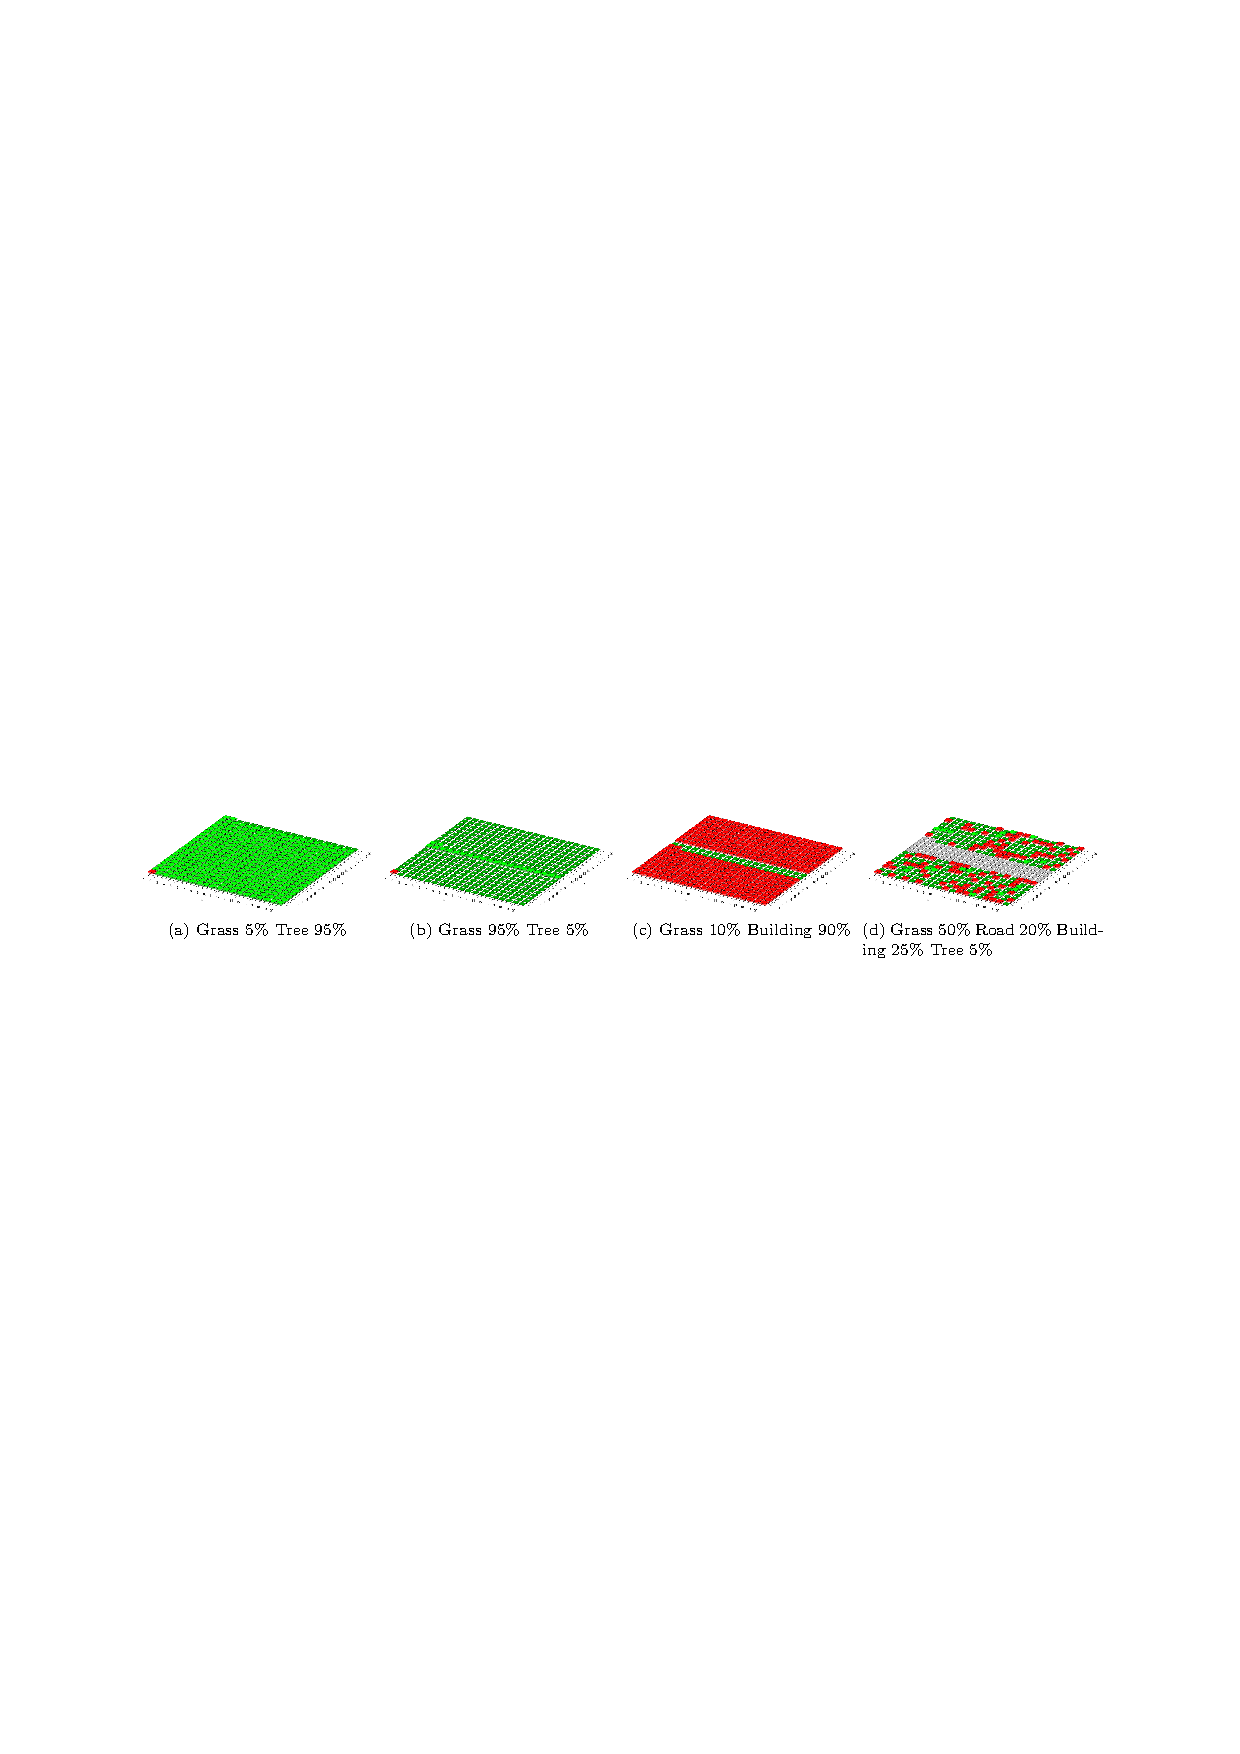
\includegraphics[page=1,trim={70 380 60 390},clip,scale=0.65]{Figures/Figures.pdf}
\caption{\bf Melbourne, creation of VTUF-3D scenarios for 9814 variations of parameters.}
 \label{fig:scenarios}
\end{figure*} 






\subsection{VTUF-3D}\label{sec:methodsvtuf}
VTUF-3D \citep{Nice2018a} was used as the micro-climate modelling tool for this study. VTUF-3D is a urban micro-climate surface energy balance model that incorporates vegetation physiological processes and shading effects. The model provides output of canyon averaged air temperature ($T_{can}$) as well as 5m resolution values for each surface of surface temperature ($T_{surf}$), mean radiant temperature ($T_{mrt}$), and universal thermal climate index ($UTCI$) (figure \ref{fig:vtufresults}). Each model run was forced by the observations of Preston in Melbourne from \cite{Coutts2007} over the days February 9-14, 2004. 

Domain mean values at ground surface level were calculated from the results from each scenario for 4 pm of February 11th for the parameters of $T_{can}$, $T_{surf}$, $T_{mrt}$, and $UTCI$ (all in $^{\circ}$C). The current forcing conditions at that point were downward shortwave (K$\downarrow$) of 501.7$Wm^{-2}$, downward longwave (L$\downarrow$) of 365.1$Wm^{-2}$, air temperature of 25.9$^{\circ}$C, vapour pressure of 1.16 $mb$, wind at 173$^{\circ}$ of 5.4 $ms^{-1}$ and air pressure of 995.5$mb$. Energy balance parameters for net radiation ($Q^{*}$), sensible fluxes ($Q_{h}$), ground flux ($Q_{g}$), and latent heat ($Q_{e}$) were also extracted, as well as shortwave and longwave up (K$\uparrow$ and L$\uparrow$) (all in $Wm^{-2}$) and canyon wind speed ($U_{road}$) (in $ms^{-1}$).

\begin{figure*}
\centering
\includegraphics[page=2,trim={75 240 60 240},clip,scale=0.55]{../Presentation/PresentationImages.pdf}
\caption{\bf Melbourne, VTUF-3D results.}
 \label{fig:vtufresults}
\end{figure*} 

\subsection{Parameter analysis}\label{sec:methodsparam}
% analysis
% ProcessMCZResults.java
% -  temperature distributions at 0m created for each completed run
%  All surfaces at 0m for each timestep, temperatures and counts of for Tsfc, Tmrt, and UTCI.
%  Ta is single value (canyon averaged) for each domain
% - All runs are combined into single data file for each timestep
%     contains temperatures and energy fluxes
% Feature importance
% /media/kerryn/87d9469d-56aa-4a1f-a62d-5f03d7599bbf/Data/VTUF-3D/Output/FeatureImportance/rf_all_runszslice.py
% feature_imporantance from RandomForestClassifier was used from scikit-learn \citep{scikit-learn}
% determine feature importance for paramaters of percentages of grass, trees, buildings, and roads, as well as average vegetation and building heights for Tair, Tsfc, Tmrt, and UTCI.




\section{Results}\label{sec:results}

%The resulting temperatures were compared to the parameters for each domain, the surface fractions and heights as well as the resulting fluxes associated with those outcomes. For $T_{can}$ (figure \ref{fig:tcanfluxes}), the greatest variations in temperatures are seen with the street fractions, the lowest temperatures seen at 50\% road area and below and slightly higher temperatures until reaching 80\%. The other fractions show an inverse (but strong) relationship

% $T_{mrt}$ (figure \ref{fig:tmrtfluxes})
%  $T_{sfc}$ (figure \ref{fig:tsfcfluxes})
%   $UTCI$ (figure \ref{fig:utcifluxes})


\begin{figure*}
\centering
\includegraphics[page=17,trim={50 300 40 295},clip,scale=1.0]{Figures/Figures.pdf}
\caption{\bf Canyon averaged air temperature ($T_{can}$) vs. domain surface fractions and heights and resulting fluxes at 4 pm of February 11, 2004.}
 \label{fig:tcanfluxes}
\end{figure*} 

\begin{figure*}
\centering
\includegraphics[page=18,trim={50 300 40 295},clip,scale=1.0]{Figures/Figures.pdf}
\caption{\bf Canyon averaged mean radiant temperature ($T_{mrt}$) vs. domain surface fractions and heights and resulting fluxes at 4 pm of February 11, 2004.}
 \label{fig:tmrtfluxes}
\end{figure*} 

\begin{figure*}
\centering
\includegraphics[page=19,trim={50 300 40 295},clip,scale=1.0]{Figures/Figures.pdf}
\caption{\bf Canyon averaged surface temperature ($T_{sfc}$) vs. domain surface fractions and heights and resulting fluxes at 4 pm of February 11, 2004.}
 \label{fig:tsfcfluxes}
\end{figure*} 

\begin{figure*}
\centering
\includegraphics[page=16,trim={50 300 40 295},clip,scale=1.0]{Figures/Figures.pdf}
\caption{\bf Canyon averaged universal thermal climate index ($UTCI$) vs. domain surface fractions and heights and resulting fluxes at 4 pm of February 11, 2004.}
 \label{fig:utcifluxes}
\end{figure*} 








\begin{figure*}
\centering
%\fbox{
\includegraphics[page=3,trim={60 220 20 225},clip,scale=0.8]{Figures/Figures.pdf}
%}
\caption{\bf T-sne clustering of UTCI.}
 \label{fig:clusterutci}
\end{figure*} 

\begin{figure*}
\centering
%\fbox{
\includegraphics[page=4,trim={60 220 20 225},clip,scale=0.8]{Figures/Figures.pdf}
%}
\caption{\bf T-sne clustering of T$_{mrt}$.}
 \label{fig:clustertmrt}
\end{figure*} 

\begin{figure*}
\centering
%\fbox{
\includegraphics[page=5,trim={60 220 20 225},clip,scale=0.8]{Figures/Figures.pdf}
%}
\caption{\bf T-sne clustering of T$_{sfc}$.}
 \label{fig:clustertsfc}
\end{figure*} 

\begin{figure*}
\centering
%\fbox{
\includegraphics[page=6,trim={60 220 20 225},clip,scale=0.8]{Figures/Figures.pdf}
%}
\caption{\bf T-sne clustering of T$_{can}$.}
 \label{fig:clustertsfc}
\end{figure*} 






\section*{References}\label{sec:ref}

  \bibliographystyle{elsarticle-harv} 
 % \bibliography{bib}
   \bibliography{BlockTypologies-EBP}


\end{document}
